
\section{The experimental platform}

This work is implemented on the robot Cog, an upper torso humanoid
\cite{brooks99cog}.  The robot has previously been applied to tasks
such as visually-guided pointing \cite{Marjanovic-96-SAB}, and
rhythmic operations such as turning a crank or driving a slinky
\cite{williamson98neural}.  Cog has two arms, each of which has six
degrees of freedom -- two per shoulder, elbow, and wrist.  The joints
are driven by series elastic actuators \cite{williamson95series} --
essentially a motor connected to its load via a spring (think strong
and torsional rather than loosely coiled).  The arm is not designed to
enact trajectories with high fidelity.  For that a very stiff arm is
preferable.  Rather, it is designed to perform well when interacting
with a poorly characterized environment, where collisions are frequent
and informative events.

\begin{figure}[tbh]
\centerline{
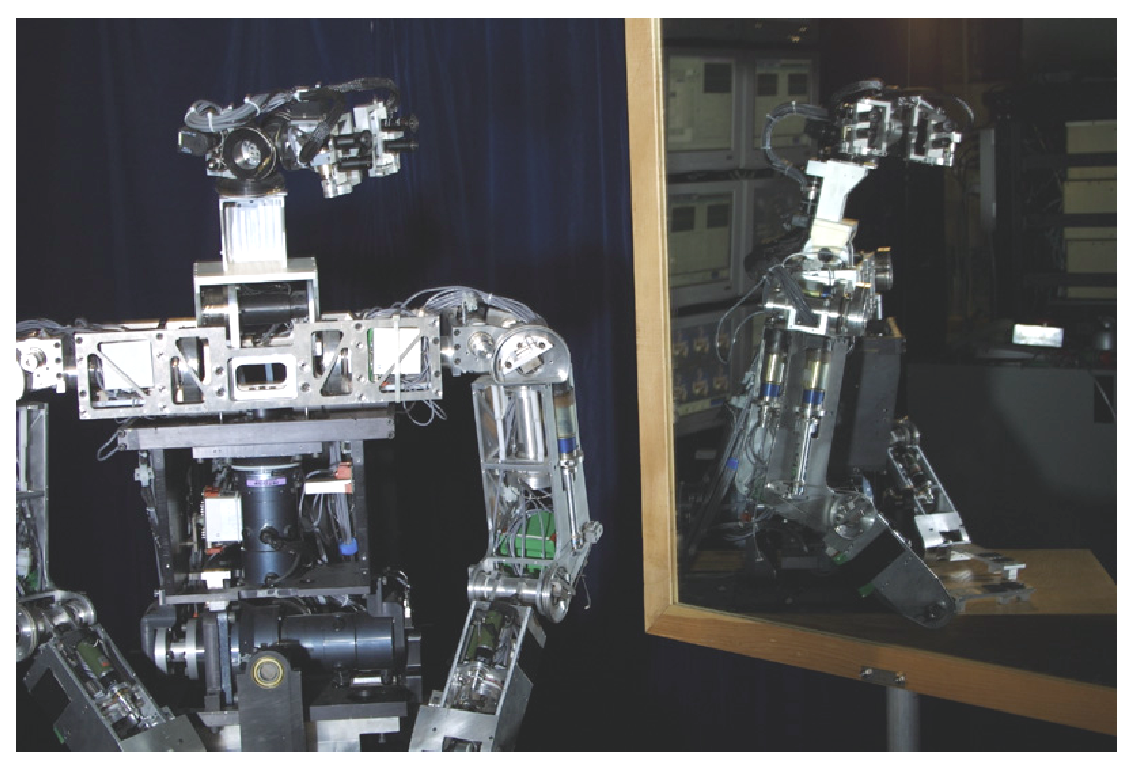
\includegraphics[width=12cm]{mirror-cog.eps}
%%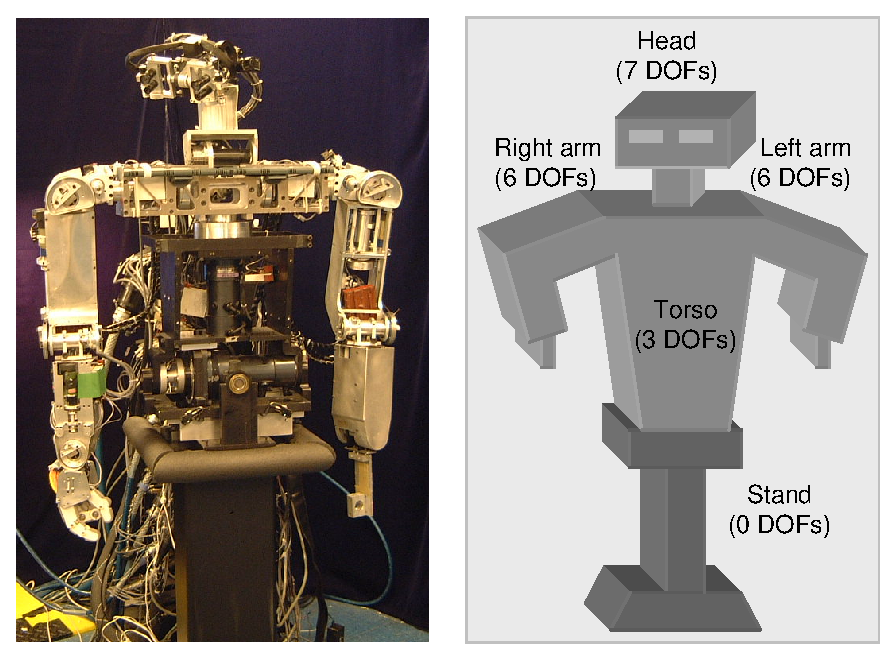
\includegraphics[width=12cm]{cog-schematic.eps}
%%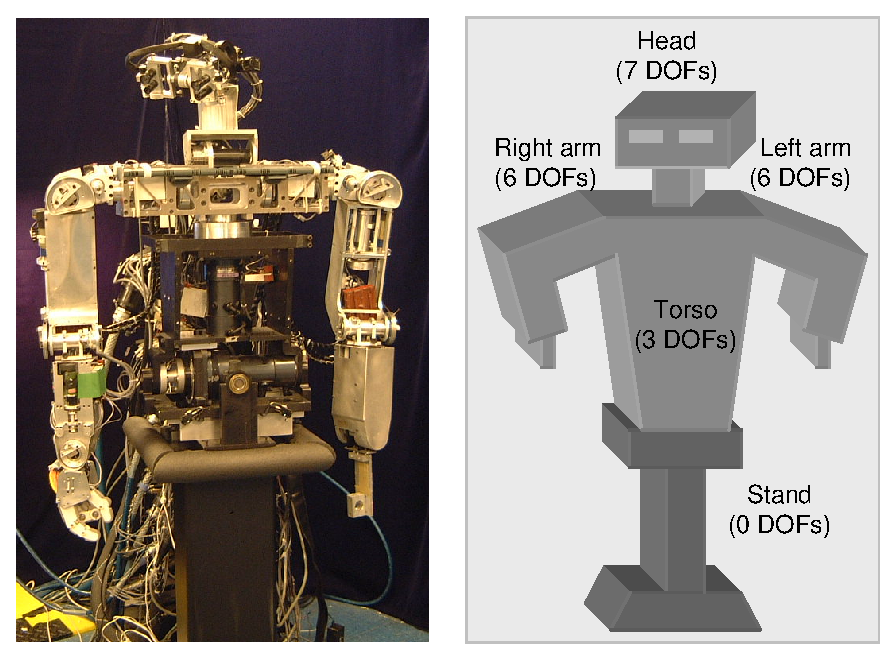
\psfig{file=cog-schematic.eps,height=2.5in,clip=,silent=}
}
\caption{ 
%
  The robot Cog, an upper-torso humanoid.  
The ultimate goal of this work is for our robot to follow chains of
causation outwards from its own simple body into the complex world.
Such an incremental process suggests that perception and action
develop together, supporting each other.
%The arms terminate
%  either in a primitive ``flipper'' or a four-fingered hand.  
% Degrees of freedom (DOFs) of the robot Cog.  The arms terminate
% either in a primitive ``flipper'' or a four-fingered hand.  
\ifverbose
The hand
  is an independent research project by Matthew Marjanovi\'{c}, and
  will not be employed or described here.  
\fi
  The head, torso, and arms
  together contain 22 degrees of freedom.
%
}
\label{fig:cog-schematic}
\end{figure}


\ifverbose
\begin{figure}[tbh]
\begin{center}
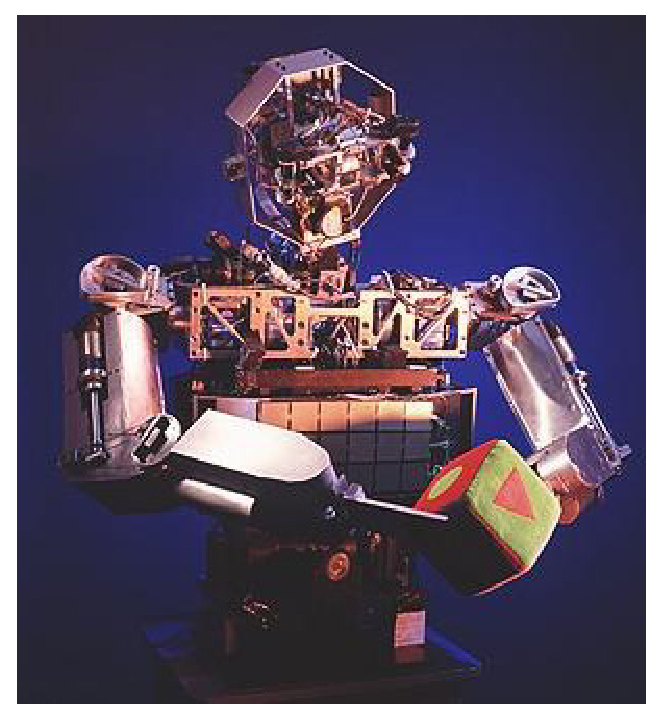
\includegraphics[height=3.5cm]{cog5-flip.eps}
\ \ \ \ 
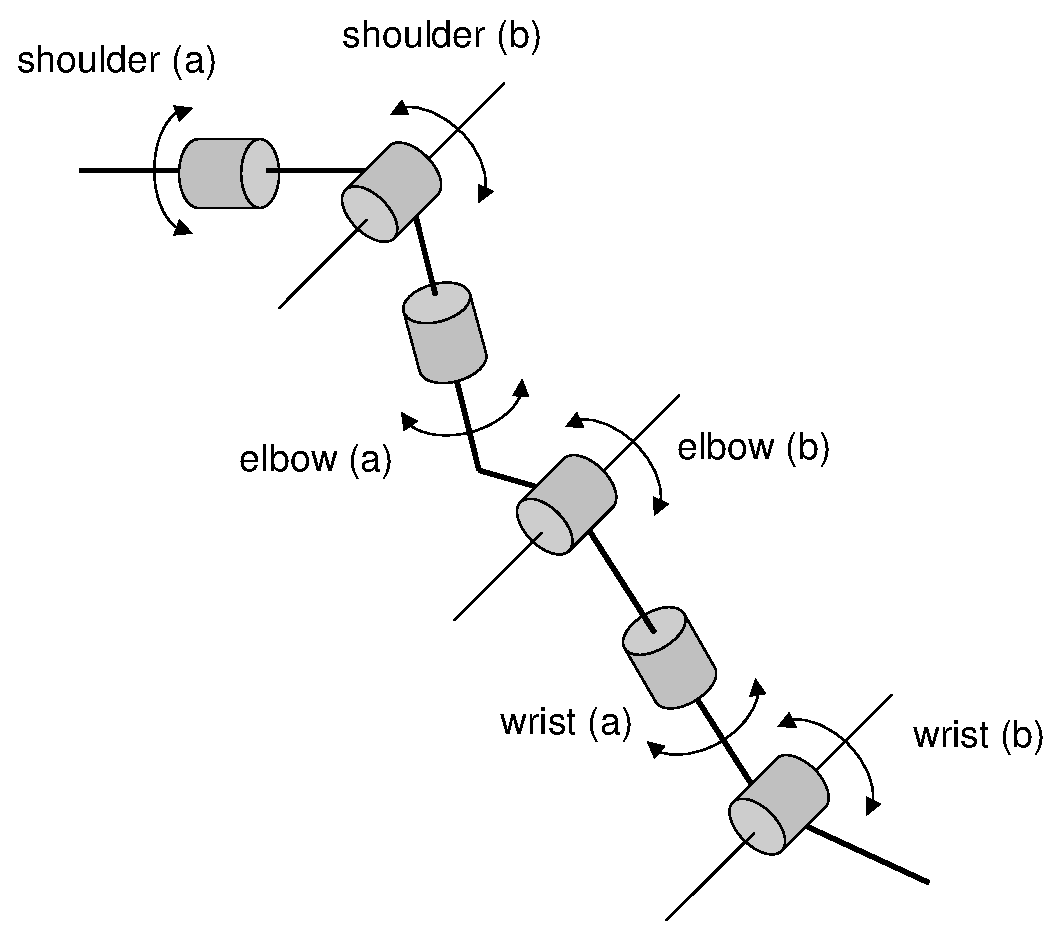
\includegraphics[height=3.5cm]{arm-motors.eps}
\caption{ 
\label{fig:arm-motors}
%
Kinematics of the arm, following \protect\cite{williamson99robot}.
There are a total of six joints, divided into a pair for each of
the shoulder, elbow, and wrist/flipper.
%
}
\end{center}
\end{figure}
\fi
